%==============================================================================
% Figure: GPS Satellite Spacetime Curvature Analogy
% Purpose: Motivational diagram illustrating practical importance of GR
% Chapter: Ch01 - Mathematical Preliminaries (Opening)
% Type: Conceptual diagram / Real-world application
%==============================================================================

\begin{figure}[htbp]
  \centering
  \resizebox{\textwidth}{!}{%
  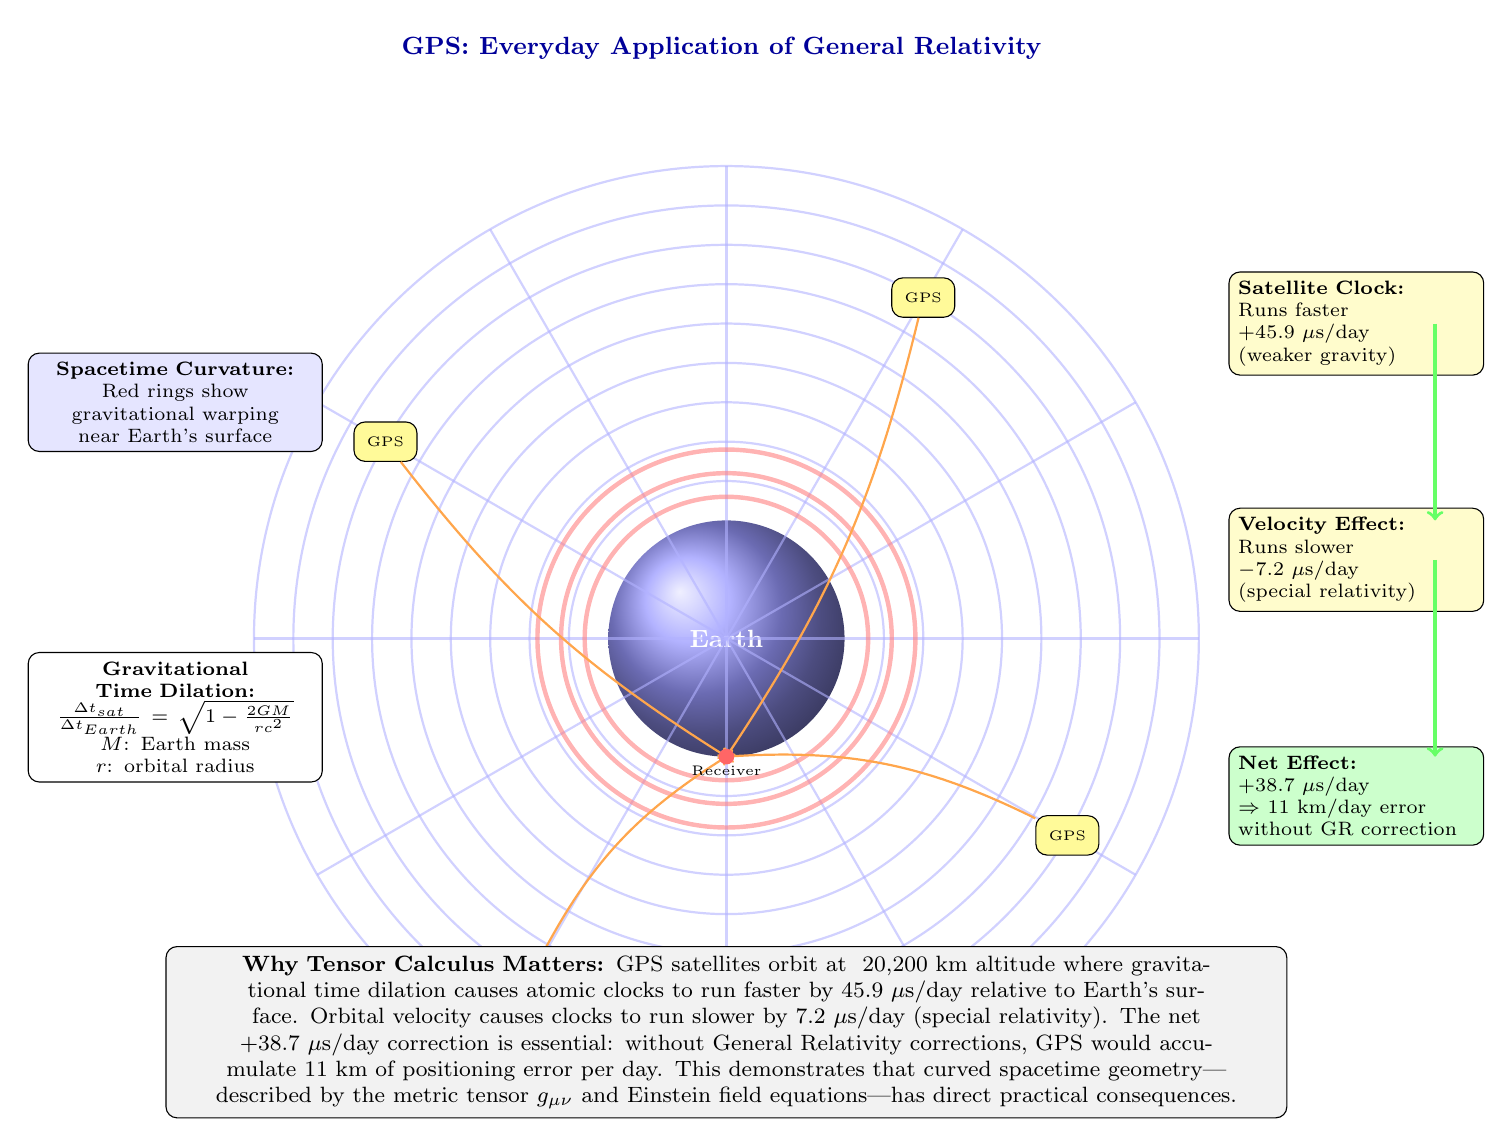
\begin{tikzpicture}[
    scale=1.0,
    satellite/.style={
      rectangle,
      rounded corners,
      minimum width=0.8cm,
      minimum height=0.5cm,
      draw=black,
      fill=gray!30,
      font=\tiny
    }
  ]

    % Earth (center)
    \shade[ball color=blue!40] (0,0) circle (1.5);
    \node[font=\small\bfseries, text=white] at (0,0) {Earth};

    % Spacetime curvature grid (warped by Earth's mass)
    % Background grid showing curvature
    \begin{scope}[opacity=0.6]
      % Curved grid lines (latitude-like)
      \foreach \r in {2, 2.5, 3, 3.5, 4, 4.5, 5, 5.5, 6} {
        \draw[blue!30, thick] (0,0) circle (\r);
      }

      % Curved grid lines (longitude-like, showing warping)
      \foreach \angle in {0, 30, 60, 90, 120, 150, 180, 210, 240, 270, 300, 330} {
        \draw[blue!30, thick] (0,0) -- (\angle:6);
      }

      % Warping intensity near Earth
      \foreach \r in {1.8, 2.1, 2.4} {
        \draw[red!50, ultra thick] (0,0) circle (\r);
      }
    \end{scope}

    % GPS satellites in orbit (Medium Earth Orbit ~20,200 km)
    % Positioned at various angles
    \node[satellite, fill=yellow!40] (sat1) at (60:5) {GPS};
    \node[satellite, fill=yellow!40] (sat2) at (150:5) {GPS};
    \node[satellite, fill=yellow!40] (sat3) at (240:5) {GPS};
    \node[satellite, fill=yellow!40] (sat4) at (330:5) {GPS};

    % Signal paths (curved due to spacetime geometry)
    \draw[->, thick, orange!70, bend left=10] (sat1) to (0,-1.5);
    \draw[->, thick, orange!70, bend right=10] (sat2) to (0,-1.5);
    \draw[->, thick, orange!70, bend left=15] (sat3) to (0,-1.5);
    \draw[->, thick, orange!70, bend right=15] (sat4) to (0,-1.5);

    % Receiver on Earth surface
    \node[circle, fill=red!60, inner sep=2pt] (receiver) at (0,-1.5) {};
    \node[font=\tiny, below] at (receiver) {Receiver};

    % Time dilation annotations
    \node[
      draw,
      rounded corners,
      fill=yellow!20,
      align=left,
      font=\scriptsize,
      text width=3cm
    ] at (8,4) {
      \textbf{Satellite Clock:}\\
      Runs faster\\
      $+45.9~\mu$s/day\\
      (weaker gravity)
    };

    \node[
      draw,
      rounded corners,
      fill=yellow!20,
      align=left,
      font=\scriptsize,
      text width=3cm
    ] at (8,1) {
      \textbf{Velocity Effect:}\\
      Runs slower\\
      $-7.2~\mu$s/day\\
      (special relativity)
    };

    \node[
      draw,
      rounded corners,
      fill=green!20,
      align=left,
      font=\scriptsize,
      text width=3cm
    ] at (8,-2) {
      \textbf{Net Effect:}\\
      $+38.7~\mu$s/day\\
      $\Rightarrow$ 11 km/day error\\
      without GR correction
    };

    % Curved spacetime annotation
    \node[
      draw,
      rounded corners,
      fill=blue!10,
      align=center,
      font=\scriptsize,
      text width=3.5cm
    ] at (-7,3) {
      \textbf{Spacetime Curvature:}\\
      Red rings show\\
      gravitational warping\\
      near Earth's surface
    };

    % Formula box
    \node[
      draw,
      rounded corners,
      fill=white,
      align=center,
      font=\scriptsize,
      text width=3.5cm
    ] at (-7,-1) {
      \textbf{Gravitational Time Dilation:}\\
      $\frac{\Delta t_{\text{sat}}}{\Delta t_{\text{Earth}}} = \sqrt{1 - \frac{2GM}{rc^2}}$\\
      $M$: Earth mass\\
      $r$: orbital radius
    };

    % Title annotation
    \node[
      font=\small\bfseries,
      text=blue!60!black,
      align=center
    ] at (0,7.5) {
      GPS: Everyday Application of General Relativity
    };

    % Bottom explanation
    \node[
      draw,
      rounded corners,
      fill=gray!10,
      text width=14cm,
      align=center,
      font=\footnotesize
    ] at (0,-5) {
      \textbf{Why Tensor Calculus Matters:} GPS satellites orbit at ~20,200 km altitude where
      gravitational time dilation causes atomic clocks to run faster by 45.9 $\mu$s/day relative
      to Earth's surface. Orbital velocity causes clocks to run slower by 7.2 $\mu$s/day
      (special relativity). The net +38.7 $\mu$s/day correction is essential: without General
      Relativity corrections, GPS would accumulate 11 km of positioning error per day. This
      demonstrates that curved spacetime geometry---described by the metric tensor $g_{\mu\nu}$
      and Einstein field equations---has direct practical consequences.
    };

    % Arrows showing correction flow
    \draw[->, very thick, green!60] (9,4) -- (9,1.5);
    \draw[->, very thick, green!60] (9,1) -- (9,-1.5);

  \end{tikzpicture}%
  }

  \caption{GPS satellite system as a practical demonstration of General Relativity. Earth's mass warps spacetime (shown by curved grid), causing gravitational time dilation: satellite clocks run faster by 45.9 $\mu$s/day in weaker gravity at orbital altitude. Orbital velocity contributes a special relativistic effect (clocks run slower by 7.2 $\mu$s/day). The net correction of +38.7 $\mu$s/day is critical---without GR-based adjustments, GPS positioning would accumulate 11 km of error daily. Orange arrows show signal paths from four satellites to ground receiver. This motivates the mathematical framework developed in Chapter 1: tensor calculus and differential geometry are not abstract formalism but essential tools for technologies we use daily.}
  \label{fig:gps-analogy}
\end{figure}
